\chapter{Introduzione}

\section{Ambito del progetto}
BLINC – Blockchain inclusiva per cittadinanze digitali è un progetto di ricerca industriale e sviluppo sperimentale emanato da Regione Piemonte
a valere sui fondi POR FESR 2014-2020 Europei. Il progetto mira a realizzare una piattaforma Blockchain per la gestione di identità digitali,
dati, transazioni di valore coinvolgendo la PA e gli operatori di servizi per i migranti.
Tutti gli attori che entrano in contatto con gli utenti potranno inserire certificazioni:
dal titolo di identità, al credito formativo, alla lettera di raccomandazione che il migrante
potrà esibire a sua discrezione, preservandone la privacy e al contempo migliorando le potenzialità di costruzione di fiducia e inclusione sociale.

Tutto ciò si integra in un progetto che permette di sperimentare soluzioni originali ad
un problema drammatico, di grande rilevanza politica e sociale, nonché esistenziale.
Essere straniero, provenire da una cultura non europea, talvolta avere una storia di fuga da situazioni insostenibili
o pericolose spesso porta a perdere l’identità formale e sociale costruita nel paese di origine, al tempo stesso la richiesta
di informazione da parte dell’ambiente circostante è maggiore. Dimenticare i propri documenti può causare problemi,
il carico burocratico e la frequenza presso gli uffici della PA sono più alti che per i cittadini italiani.
Attraverso la Blockchain sarà possibile strutturare tecnologie per la fiducia, atte a colmare quel gap di informazione che frena
i processi di inclusione dei migranti, senza portare a stigmatizzazioni o discriminazioni nel diritto alla privacy.

Il funzionamento dell’applicazione base proposta è semplice, un portadocumenti virtuale che contiene certificati auto-generati 
(ad esempio a partire da documenti cartacei o per dichiarazione) accanto a documenti generati dei servizi privati e pubblici con cui il migrante viene in contatto.
Il portadocumenti è accessibile da qualsiasi dispositivo, ma pensato per il mobile, con interfacce semplificate che rendono
l’uso compatibile con scarse competenze digitali.

Un altro aspetto fondamentale del prodotto è la gestione granulare della privacy: il portadocumenti non può essere consultato
nella sua interezza, ma, utilizzando tecnologie Blockchain pensate per i record sanitari, l’utente potrà decidere quali certificati ne fanno parte.
L’iniziativa si colloca nel contesto della sharing economy ed il progetto valuterà possibili integrazioni con altre operazioni Blockchain
condotte dall’Università di Torino, in particolar modo nel campo delle valute sociali locali e del sistema di protezione sociale,
con il progetto Co-City riguardante il coinvolgimento diretto (patti di collaborazione) dei cittadini attivi nella generazione di servizi negli spazi urbani inutilizzati.

\section{Descrizione dell'azienda}
Consoft Sistemi\footnote{Consoft Sistemi: https://www.consoft.it} è presente sul mercato ICT dal 1986 con sedi a Milano, Torino, Genova, Roma e Tunisi.
Accanto alla capogruppo sono attive altre 4 società: CS InIT, specializzata nello scouting e distribuzione di soluzioni software, Consoft Consulting 
focalizzata sulla PA, Consoft Sistemi MEA e C\&A Soft Consulting per espandere l’offerta della capogruppo nel mercato nord-africano e medio-orientale. 
Il Gruppo Consoft ha focalizzato la propria offerta su alcune aree tematiche, prevalentemente focalizzate sul tema della Digital Transformation nell’ambito
delle quali è in grado di realizzare soluzioni “end to end” per i propri Clienti attraverso attività di consulenza, formazione, realizzazione di soluzioni
integrate ed erogazione di servizi in insourcing/outsourcing.

Ha ottenuto la Certificazione ISO 27001 ed ha un Sistema di Gestione Qualità certificato UNI EN ISO 9001:2008.
Tra le aree di specializzazione tecnologica
annovera DevOps e Testing, Analytics \& Big Data, Cyber Security e Internet of Things.

Consoft Sistemi è parte del CDA del Cluster Tecnologie
per le Smart Cities \& Communities Lombardia, è membro di Assolombarda ed Assintel
(tramite CS\_InIT) ed attiva nei progetti di innovazione proposti dagli Enti.
Ha fatto parte dell’Osservatorio Internet of things e Osservatorio Big Data del MIP, è membro IOTitaly.

Consoft Sistemi come partner tecnologico collabora attivamente a progetti di ricerca sia regionali che nazionali
ed europei con l’obiettivo di studiare e realizzare soluzioni che arricchiscano il mercato con ulteriori
componenti ICT sviluppati a partire dalla realtà progettuale proposta,
basati pertanto su un'esperienza che ne abbia già stimato il grado di fattibilità e sostenibilità economica.

Le attività di R\&D inoltre, permettono di creare ulteriori contatti tra aziende di dimensioni diversificate, centri di ricerca,
università ed operatori di settore per costruire un’offerta di servizi più completi e competitivi e per consentire l’utilizzo sinergico di risorse
nell'ottica di un complessivo aumento di efficienza ed efficacia.

L’Innovazione sociale attraverso il miglioramento della qualità della vita è tra i temi di maggiore interesse di Consoft
Sistemi ed è in questo ambito
che si colloca il progetto su cui è stato condotto e sviluppato il tirocinio.

\section{Architettura generale del progetto}

\begin{figure}[!ht]
    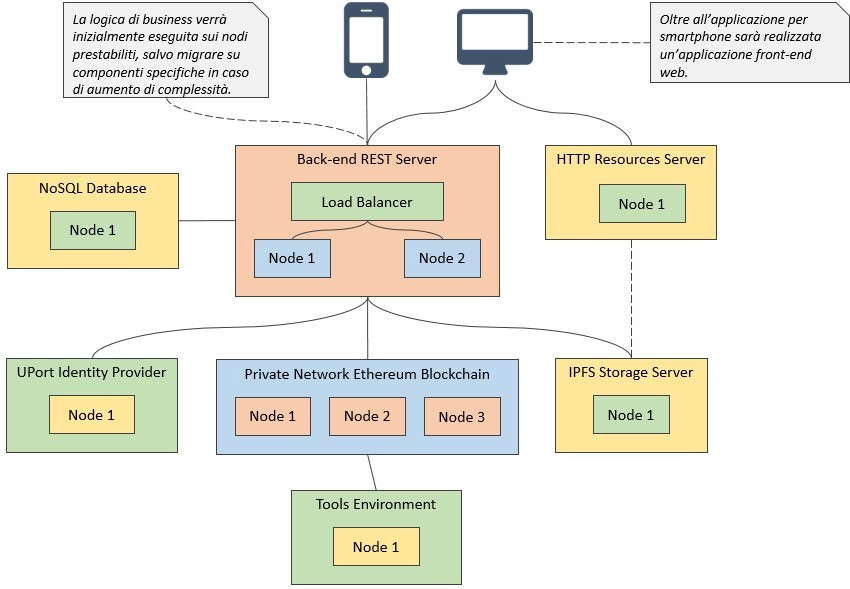
\includegraphics[width=\linewidth]{diagrammaarchitettura}
    \caption{Diagramma dell'architettura di BLINC.}
    \label{fig:diagrammaarchitettura}
\end{figure}

L’architettura è composta da (da sinistra a destra, dall’alto in basso):
\begin{itemize}
    \item Applicazione mobile (native Android ed iOS) e web app: servono ai migranti ed agli operatori
    per interfacciarsi ai servizi di BLINC.
    Comunicano con i server REST e di risorse tramite chiamate ad API
    \item Database NoSQL (MongoDB\footnote{MongoDB: https://www.mongodb.com/}): necessario per memorizzare informazioni e wallet
    criptati degli utenti
    \item Server di back-end (Loopback\footnote{LoopBack: https://loopback.io/}, framework di creazione di API basato su NodeJS): espone gli endpoint API richiamabili
    dai client, contiene la business logic e accede alla rete Ethereum per interagire
    con le identità dei migranti e effettuare dichiarazioni ed endorsement sulle generalità e documenti da essi caricati
    \item HTTP Resources Server: necessario per servire risorse statiche (immagini, documenti…) ai client
    \item uPort Identity Provider: insieme di \emph{smart contract} uPort distribuiti sui nodi Ethereum sottostanti che rendono
    possibile la creazione e gestione di identità e di attestazioni relative ad esse.
    \item Blockchain Privata Ethereum: insieme di macchine che eseguono istanze del client Ethereum Geth.
    \item IPFS\footnote{InterPlanetary File System: https://ipfs.io/} Storage Server: un nodo IPFS, sistema di storage decentralizzato, necessario per salvare i 
    documenti cifrati degli utenti.
    \item Tools environment: strumenti di monitoraggio della chain privata Ethereum citata in precedenza,
    in particolare un \emph{block explorer} ed un
    \emph{netstats}, che permettono rispettivamente di visualizzare le transazioni incluse per blocco
    e di avere una visione di insieme sulla rete Ethereum privata,
    tra cui la difficoltà della rete, i nodi che partecipano ad essa e l'uptime.
\end{itemize}

\subsection{Soluzione tecnologica}

\begin{figure}[!ht]
    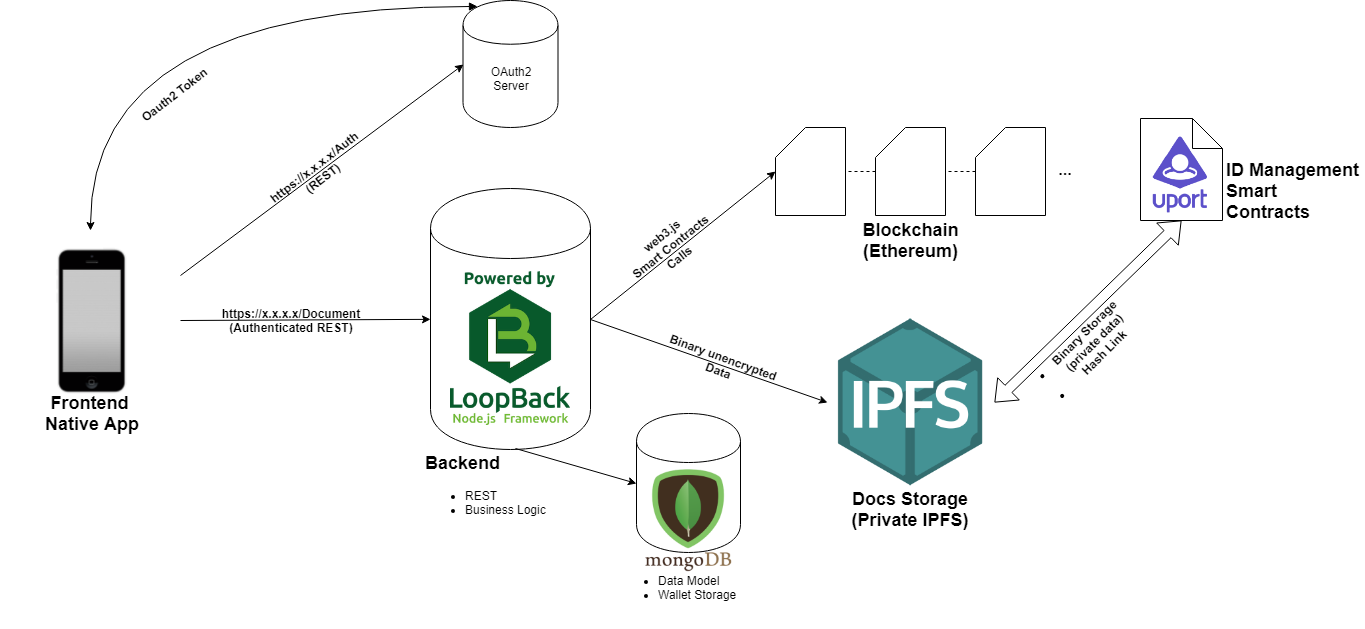
\includegraphics[width=\linewidth]{soluzionetecnologica}
    \caption{Soluzione tecnologica per BLINC.}
    \label{fig:soluzionetecnologica}
\end{figure}

Data l’immaturità del SDK di uPort che non ha permesso la creazione del wallet del migrante sul proprio telefono, la prima versione 
dell’architettura e di flusso di accesso ai servizi include elementi provvisori come l’OAuth server
(basato su login tramite e-mail e password e centralizzato, 
entrambe cose che si vorrebbero evitare) e MongoDB (che contiene i wallet degli utenti criptati).	
In questa prima versione il flusso d’interazione base è quindi questo:

\subsubsection{Utente registrato}

L’utente apre l’applicazione di BLINC, inserisce e-mail/nome utente e password che vengono inviati all’OAuth server:
se e-mail/nome utente esistono e la password associata è corretta viene restituito un token di autorizzazione
tramite il quale l’utente
potrà accedere alle API protette del backend.

Grazie al token ricevuto, l’utente può accedere innanzitutto alla propria identità uPort, salvata su database, 
per caricare documenti e verificare attestazioni sulle proprie credenziali e sui propri documenti.

\subsubsection{Utente non registrato}

Al primo accesso all’app BLINC il migrante inserisce informazioni base (nome, cognome, telefono…),
la propria e-mail ed una password. Queste ultime vengono salvate sull’OAuth server per i login successivi, 
l’identità viene creata con le informazioni inserite in precedenza tramite le librerie apposite di uPort 
e salvata su MongoDB, dove viene anche creato, criptato e salvato il wallet Ethereum dell’utente,
composto da una coppia di chiavi ed un indirizzo Ethereum, ricavato dalla chiave pubblica.

\section{Obbiettivo della tesi}

L'obbiettivo della tesi è quello di spiegare in dettaglio il mio lavoro di ricerca ed applicazione
di soluzioni blockchain e di identità digitale decentralizzata nell'ambito del progetto BLINC.

Gran parte del mio tirocinio è stata dedicata alla ricerca e poi alla sperimentazione delle tecnologie
abilitanti: in primissimo luogo ho studiato cos'è una blockchain \cite{WEBSITE:4} per poi iniziare l'approfondimento
su Ethereum, la blockchain definita come \emph{world computer} \cite{WEBSITE:5}. 
Da qui le prime sperimentazioni: installazione del client Ethereum 
Geth\footnote{Go Ethereum: https://geth.ethereum.org/} con invio di transazioni e deploy di smart contract
prima da linea di comando e poi tramite la libreria JavaScript 
web3.js\footnote{web3.js: https://github.com/ethereum/web3.js}.
Una volta preso confidenza con i concetti e gli strumenti base per poter comprendere e lavorare su
Ethereum ho iniziato a focalizzarmi sulla parte di mia competenza per il progetto: l'identità digitale.
Dopo una ricerca iniziale sull'identità a sovranità personale ho approfondito la soluzione specifica
più adatta a BLINC selezionata dopo una scelta condivisa tra tutte le parti interessate nel progetto, ovvero
uPort\footnote{uPort: https://uport.me}.
In seguito ad uno studio dell'architettura e delle librerie che uPort a disposizione, ne è stata
scelta una che venisse incontro alle nostre esigenze, almeno per una prima versione di BLINC.
Da qui inizia il lavoro pratico sul progetto in collaborazione con i miei colleghi tirocinanti,
ovvero lo sviluppo di una prima versione del sistema secondo l'architettura descritta precedentemente:
in particolare mi sono occupato della creazione di endpoint API in NodeJS per la creazione e gestione
di identità ed attestazioni su di esse sfruttando la libreria \texttt{uport-js-client}.